\chapter{Exploration of Alternative Systems}
\section{Introduction}

There are three broad classes of material that have been explored as aero-engine blade material: metal alloys, ceramics and intermetallics.  Some metal alloys have excellent room temperature properties, but have much lower homologous temperatures than intermetallics and ceramics. Consequently, metal alloys have lower operating capabilities than intermetallics and ceramics, and are unsuitable for higher temperature operation.  

This leaves us with two categories of systems that have suitable candidates for high temperature applications. The first category are systems based on ceramics. The options include: monolithic ceramics and ceramic matrix composites (CMCs). The second category of systems are based on intermetallic phases. The options are: monolithic or multi-phase intermetallics, metal-intermetallic materials. 

The academic community has identified various ceramic systems that have potential as successors to nickel-base superalloys.  Ceramics have very high melting points and homologous temperatures; some have the ability to retain strength at temperatures beyond 2000\celsius\ (Figure \ref{fig:CeramicsIntermetallics}). However, the greatest hurdle faced by both monolithic ceramics and CMCs is their intrinsic lack of room temperature toughness ~\cite{evans80}.  Due to the nature of their atomic bonds, it is unlikely that this can be surmounted. For this reason, we will not be exploring ceramics further in this work.

Several monolithic and multi-phase intermetallic systems are seen to offer a compromise between the room temperature robustness of superalloys and the high temperature capabilities of ceramics. Their room temperature toughnesses, however, are insufficient, and intermetallic systems will not be considered in this work. Thus, by process of elimination, this thesis will focus on the options available in the realm of metal-intermetallic composites.
%
\begin{figure}[H]
\begin{center}
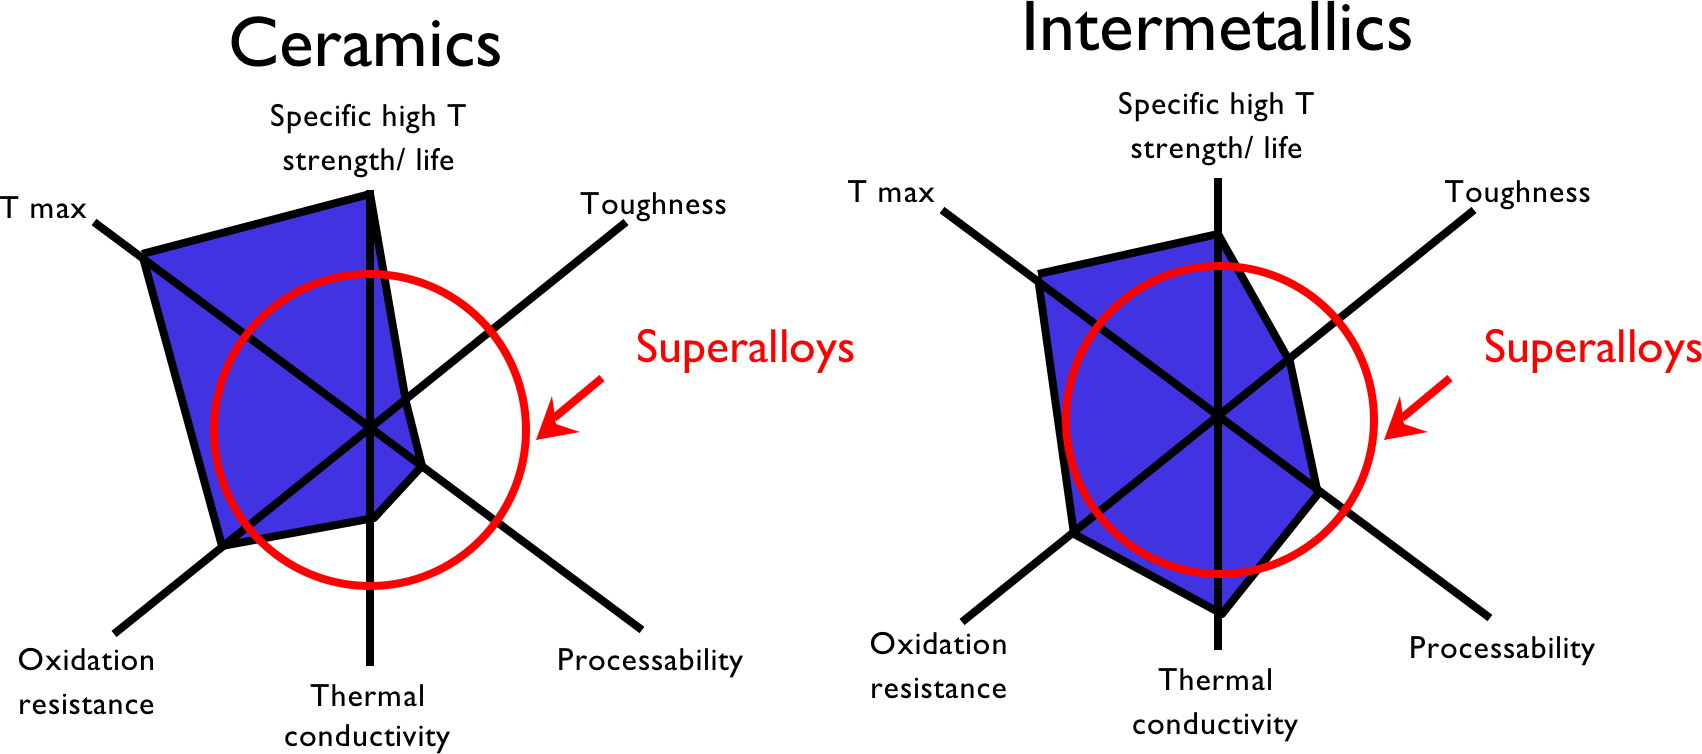
\includegraphics[width=\textwidth]{CeramicsIntermetallics}
\caption{Properties of ceramics and intermetallics compared to superalloys. (adapted from Superalloys 1980) }\label{fig:CeramicsIntermetallics}
\end{center}
\end{figure}
%
%There are ceramic systems that are very oxidation resistant than superalloys, which is desirable.Some intermetallic systems can be seen to offer a compromise between the room temperature robustness of superalloys and the high temperature capabilities of ceramics. 
\section{Exploration of Alternative Metal-Intermetallic Systems}

Resistance to oxidation during exposure between room and operating temperatures is a neccessity for blade materials.  This would prevent catastrophic failure through runaway oxidation from occuring.  Whilst coatings may be used to protect the alloy, the alloy must possess sufficient oxidation resistance to survive between service intervals, if the coating should fail in service. The three oxides through which oxygen has the lowest permeability are those of aluminium, chromium and silicon.  To base our alloy system on one of these elements would be a sound start. With the success enjoyed by nickel-base superalloys as high temperature materials, there was a natural progression for research to concentrate on select aluminides, such as Ni$_3$Al, NiAl and FeAl, in the 1980s ~\cite{cotton93, miracle94a, walston93, white89}.  Extensive efforts undertaken to improve their high temperature mechanical properties did not lead to increases in creep resistance.  Aluminides are believed to be unlikely to achieve higher temperature capabilities than nickel-base superalloys.

There has been some work done on developing alumina-forming superalloys based on platinum group metals (PGMs), such as platinum, iridium and rhodium ~\cite{wenderoth05, mitarai98, mitarai97}. These alloys are similar to nickel-base superalloys, and have a solid solution matrix with a loading-bearing intermetallic L1$_2$ phase. These alloys melt at higher temperatures than nickel-base superalloys and have the potential to operate at temperatures that are several hundred degrees higher than current superalloys. Although this approach has met with some success, these materials are three times denser than nickel-base superalloys and are prohibitively expensive.  Their density make them unsuitable for moving parts, but they may be suitable for projects that operate on an essentially unlimited budget, such as inter-planetary rocketry missions, but it is difficult to justify the costs that would be incurred for use in commercial jet engines.  We believe that there are better development options available, and will not be exploring PGM superalloys further in this work. 

Chromium oxide is known to be excellent for corrosion resistance; in fact, the principle method for making stainless steels stainless is through the addition of chromium.  Chromium oxide, however, has the unfortunate characteristic of volatilising at temperatures above 950\celsius\ ~\cite{perez02}, and is typically deemed unsuitable as the means of protection for operating temperatures that are to exceed 1100\celsius.

Silicon dioxide is stable up to 1650\celsius ~\cite{hallstedt92}, which is substantially higher than the target temperature capability of 1200\celsius .  Its adhesion to the underlying substrate, however, has not been quantified.  Given the historical preference for alumina formers, it is suspected that silica may not be as adherent as alumina.  for these reasons, attention has predominantly been focused on the development of refractory metal silicides. Silicides have low to moderate densities, exhibit excellent high temperature oxidation resistance ~\cite{brady00}.  Several systems have been shown to demonstrate temperature capabilities that are almost 200\celsius\ higher than nickel-base superalloys ~\cite{schneibel03, sadananda99}.  However, there are significant deficiencies that must be overcome if these materials are to achieve widespread usage. These include poor room temperature ductility, poor oxidation resistance at intermediate temperatures and in the prescence of water vapour. As such, it remains uncertain whether these materials will ultimately be successful. Additionally, the possibility that other parties, such as competing aeroengine manufacturers, are developing alternative materials based on systems other than those that have been published in the open literature cannot be dismissed. An aim of this dissertation is to conduct an exploration of silicide systems to identify those with the potential for high temperature operation, have alloying capabilities with one another, and have the potential to exhibit damage tolerance at room temperature.
%
\begin{figure}[H]
\begin{center}
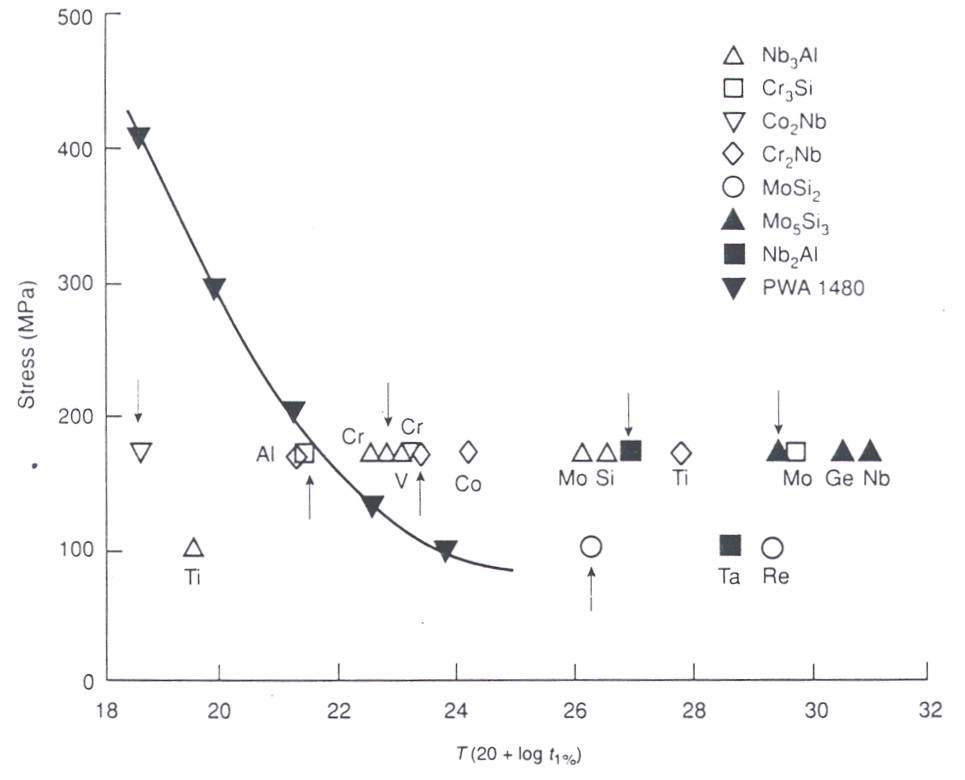
\includegraphics[width=13cm]{LMplotforintermetallics}
\caption{Larson-Miller plot of the stress for 1\% creep in steady state, comparing creep resistances of intermetallic compounds and their alloys against a single crystal superalloy, PWA 1480 ~\cite{anton89, anton89b, shah95}.}
\label{fig:LMplotforintermetallics}
\end{center}
\end{figure}
%
\subsection{Exploration of Refractory Metal Silicide Systems as Alternative Blade Material}
In the last decade, the academic community has given molybdenum and niobium silicides the most attention.  Although they out-perform nickel-base superalloys in high temperature creep, they form non-protective oxides at intermediate temperature ~\cite{tomasi97, yanagihara96, sauthoff88, ochiai06, mitra06, miracle94}.  More alloying will have to be done to improve their oxidation resistance.  There is also limited literature on chromium and vanadium silicides.
%
 			
\subsection{Molybdenum Silicides}
There are three molybdenum silicides in the Mo--Si binary: Mo$_3$Si, Mo$_5$Si$_3$ and MoSi$_2$ (Figure: \ref{fig:MoSi}) ~\cite{svechnikov70}. Molybdenum has a density of 10.28 \gram\usk\centi\rpcubic\meter, and Mo$_3$Si has a density of 8.4 \gram\usk\centi\rpcubic\meter.
Molybdenum silicides have been heavily researched as they have high melting points of above 2000\celsius\ ~\cite{svechnikov70}, high temperature strength retention, and good high temperature oxidation resistance .  However, they are suceptible to ``pesting", which is catastrophic runaway oxidation that occurs at intermediate temperatures \cite{shah92}. This can be observed for MoSi$_2$ in Figure \ref{fig:MoSi2_oxidation}. 
%
\vspace{6mm}
\begin{figure}[H]
\begin{center}
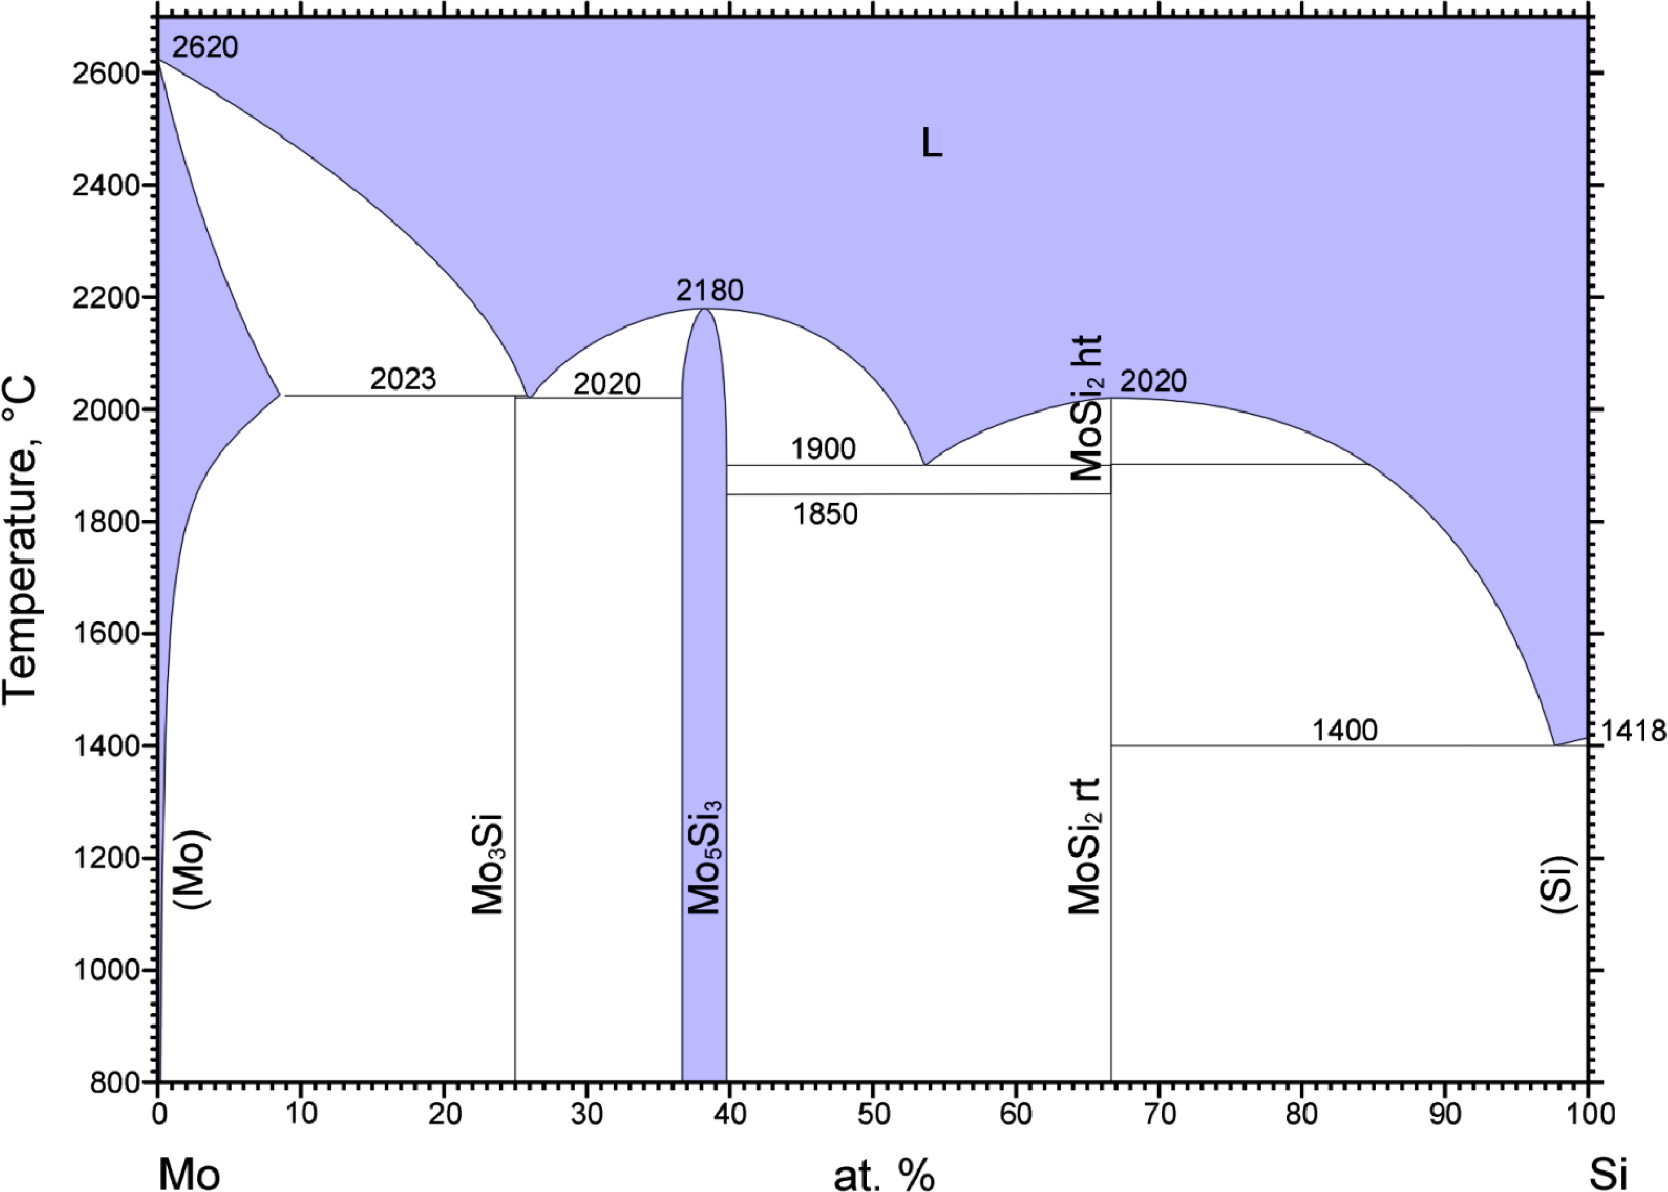
\includegraphics[width=15cm]{MoSi}
\caption{The Mo-Si binary phase diagram ~\cite{svechnikov70}}
\label{fig:MoSi}
\end{center}
\end{figure}
%
\vspace{6mm}
\begin{figure}[H]
\begin{center}
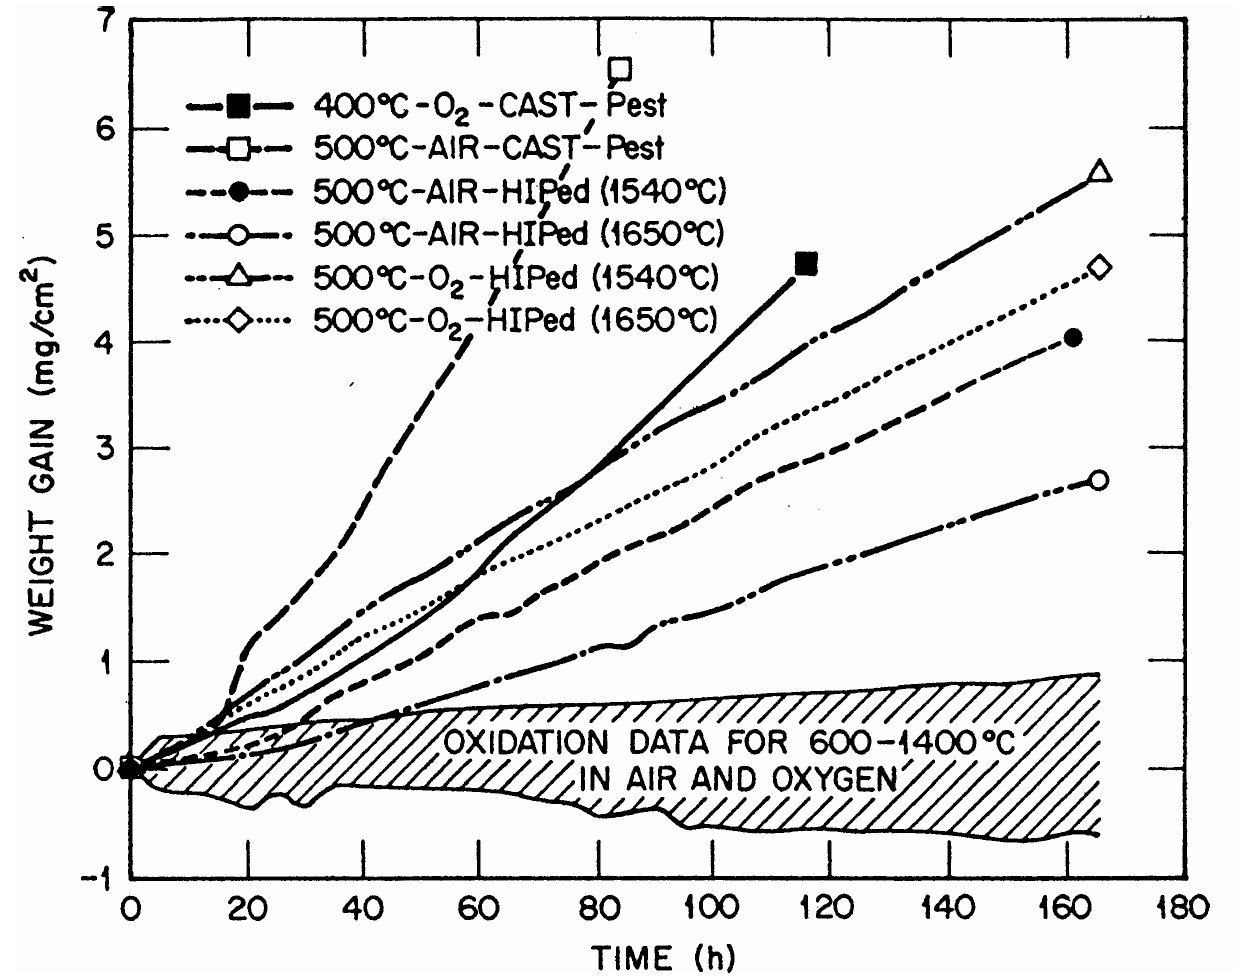
\includegraphics[width=10cm]{MoSi2_oxidation}
\caption{Mass change of MoSi$_2$ during oxidation at temperatures between 400--1400\celsius. ~\cite{inui00}}
\label{fig:MoSi2_oxidation}
\end{center}
\end{figure}
\vspace{-5mm}
%
Mo$_5$Si$_3$ has been quite heavily researched thus far, as it has the highest melting point in the Mo--Si binary ~\cite{svechnikov70}, but it has poor room temperature fracture toughness of 3 \mega\pascal\,m$^\frac{1}{2}$ and poor oxidative properties at intermediate and high temperatures ~\cite{akinc99, anton89, anton89b}. Akinc has reported 3 at.\% boron additions to Mo$_5$Si$_3$ improves its oxidative properties between 800 -- 1500\celsius\ by as much as 5 orders of magnitude (Figure \ref{fig:Mo5Si3_oxidation}).  During the initial onset of oxidation, a boro-silicate glass forms in competition with MoO$_3$.  MoO$_3$ is the cause of catastrophic oxidation of Mo$_5$Si$_3$; it sublimes at 750\celsius\ ~\cite{brewer90} and is non-protective.  The boro-silicate glass experiences viscous flow at 1000\celsius\ and promotes closure of submicron scale porosity left behind due to MoO$_3$ volatilisation, minimising subsequent oxidation of Mo into MoO$_3$Si (Figure \ref{fig:MoSi_oxidationpictures}) ~\cite{akinc99}. 
% 
\begin{figure}[H]
\begin{center}
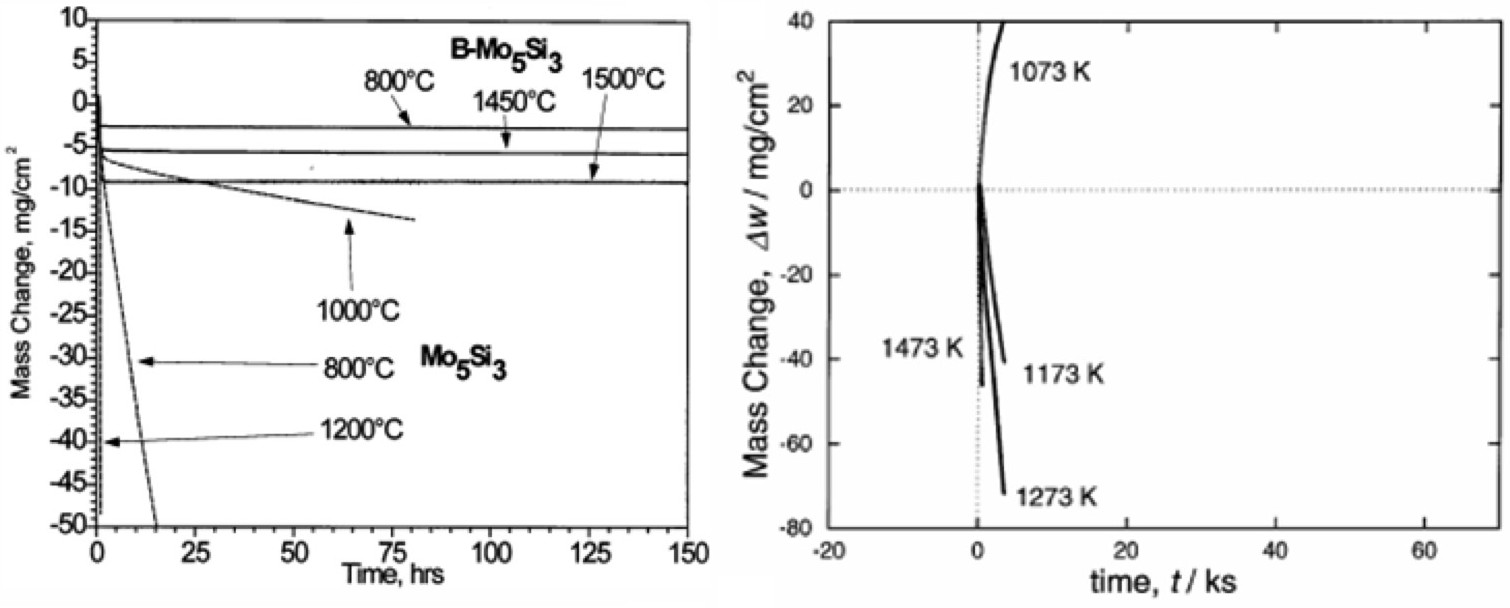
\includegraphics[width=.9\textwidth]{Mo5Si3_oxidation}
\vspace{-.3cm}
\caption{Mass change of Mo$_5$Si$_3$ during oxidation at temperatures between 800--1500\celsius\ ~\cite{akinc99}.}\label{fig:Mo5Si3_oxidation}
\end{center}
\end{figure}
\vspace{-.5cm}
%
\begin{figure}[H]
\begin{center}
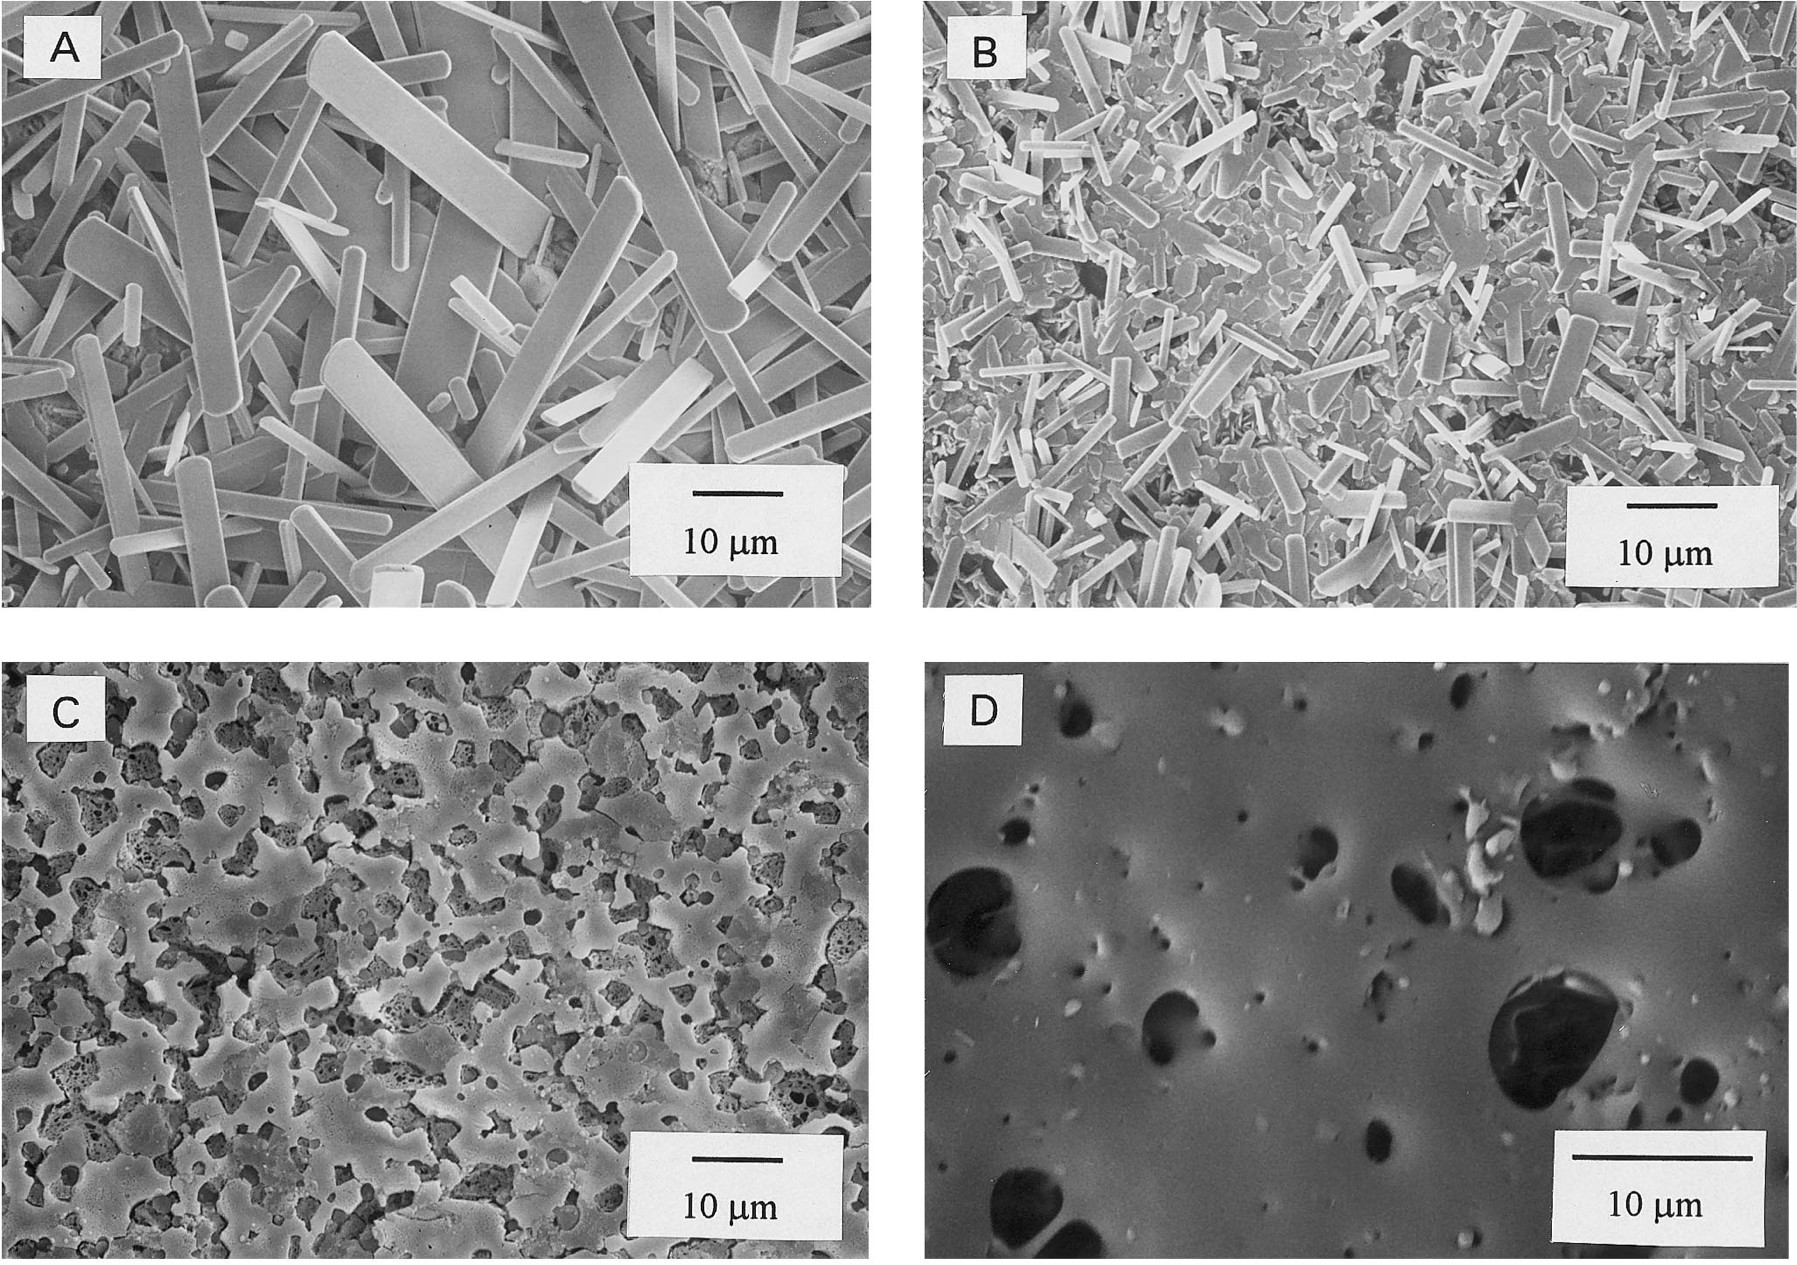
\includegraphics[width=.7\textwidth]{MoSi_oxidationpictures}
\vspace{-2mm}
\caption{SEM micrographs of the transition of the initial oxide from MoO$_3$ oxide to a boro-silicate glass ~\cite{akinc99}.}\label{fig:MoSi_oxidationpictures}
\end{center}
\end{figure}
\vspace{-1cm}
%
The Mo$_5$SiB$_2$ phase (Figure \ref{fig:T2structure}) has been a focus of great interest to the high temperature materials community due to its unparallelled creep properties at 1500\celsius\ ~\cite{hayashi04, ito01}, which is a 400\celsius\ increase in creep capability over nickel superalloys.  At 1300\celsius, its creep rate is about 3 orders of magnitude lower than an ideally oriented MoSi$_2$ sample. Alur reported that the T2 particles in a solid solution matrix alloy, when subject to compression creep at different temperatures and strain rates, show a range of deformation behaviour ~\cite{alur04}. Brittle fracture, plastic deformation and elastic deformation were all observed. 

Nowotny et al. identified Mo$_5$SiB$_2$ in a 1600\celsius\ isothermal section of the ternary in 1957(Figure \ref{fig:MoSiB_1600}) ~\cite{nowotny57}, this phase diagram has recently been revised by Nunes et al. ~\cite{nunes97}. A Mo--Mo$_5$SiB$_2$ pseudo-binary phase diagram has also been constructed by Yoshimi et al. Figure \ref{fig:Mo-Mo5SiB2}) ~\cite{yoshimi03}.

Perepezko explored microstructure control to manufacture Mo-Mo$_5$SiB$_2$ and Mo-Mo$_3$Si-Mo$_5$SiB$_2$ for ultrahigh temperature applications ~\cite{perepezko01}. The ternary eutectic is difficult to attain through ingot castings, as solidification segregation causes very stable borides and silicides to form instead.  Also, the liquidus surfaces for Mo$_3$Si and T2 around the ternary eutectic region are shallow (Figure \ref{fig:MoSiB_liquidus}). The invariant eutectic can be by-passed during non-equilibrium solidification. Mo$_3$Si and T2 would form instead, and there will be very little toughening component in the microstructure (Figures \ref{fig:Mo16Si8B} and \ref{fig:MoSiB_witheutectic}).%
%
\vspace{8mm}
\begin{figure}[H]
\begin{center}
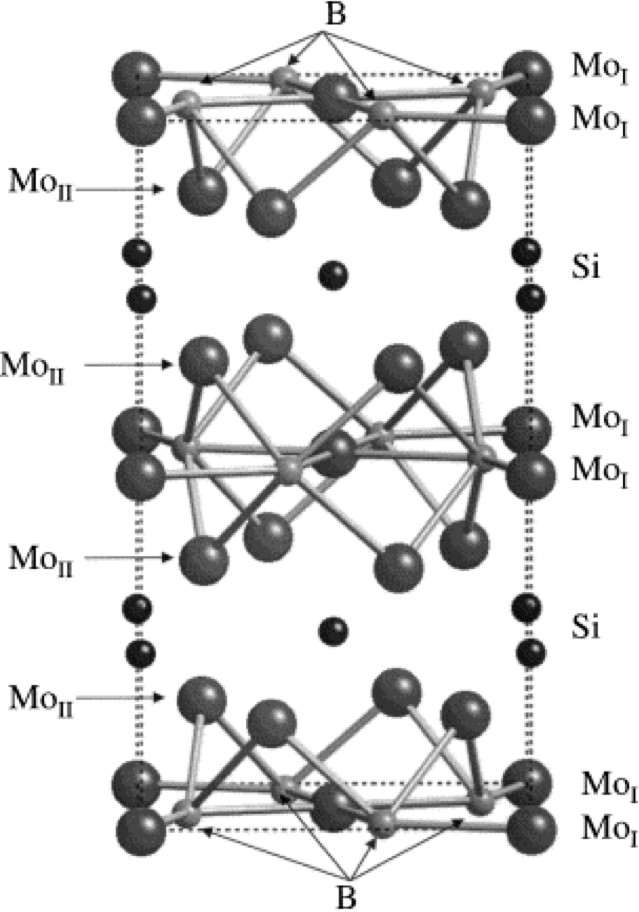
\includegraphics{T2structure}
\caption{The crystal structure of Mo$_5$SiB$_2$ ~\cite{rawn01}. }
\label{fig:T2structure}
\end{center}
\end{figure}
\vspace{-.2cm}
%It has superior compression creep properties, and out-performs current commercial nickel-base superalloys by 400\celsius\ ~\cite{perepezko01}. However, its layered crystal structure may result in poor properties in shear, akin to that in graphite. 
%
\begin{figure}[H]
\begin{center}
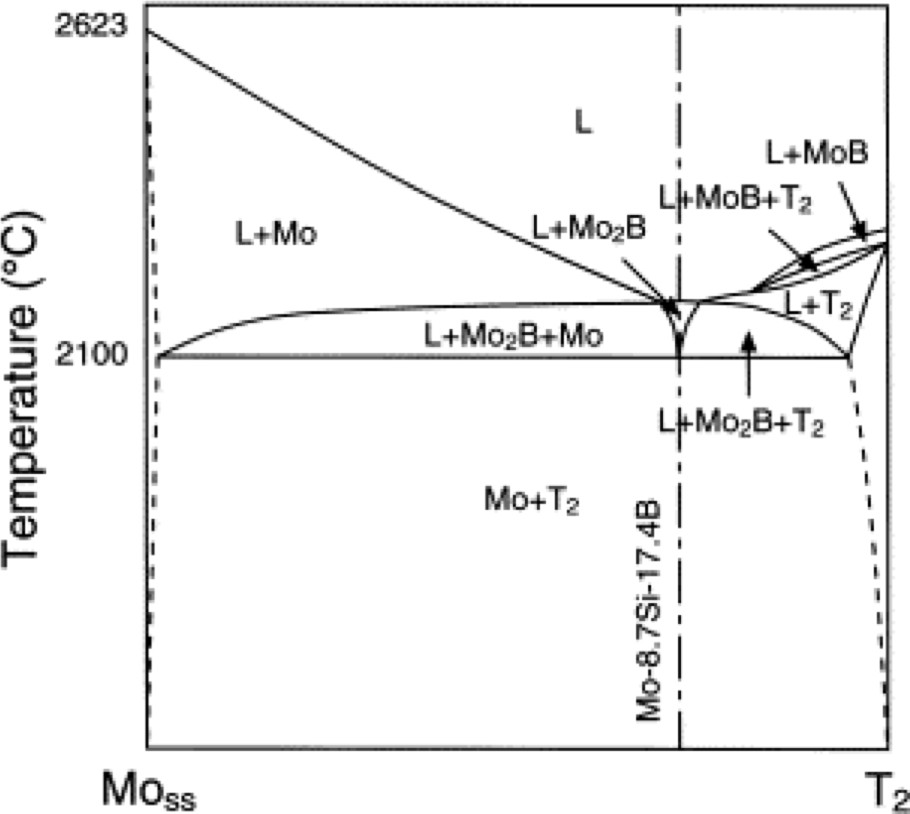
\includegraphics[width=8cm]{Mo-Mo5SiB2}
\caption{Mo--Mo$_5$SiB$_2$ pseudo binary phase diagram ~\cite{yoshimi03}.}
\label{fig:Mo-Mo5SiB2}
\end{center}
\end{figure}
%
\begin{figure}[H]
\begin{center}
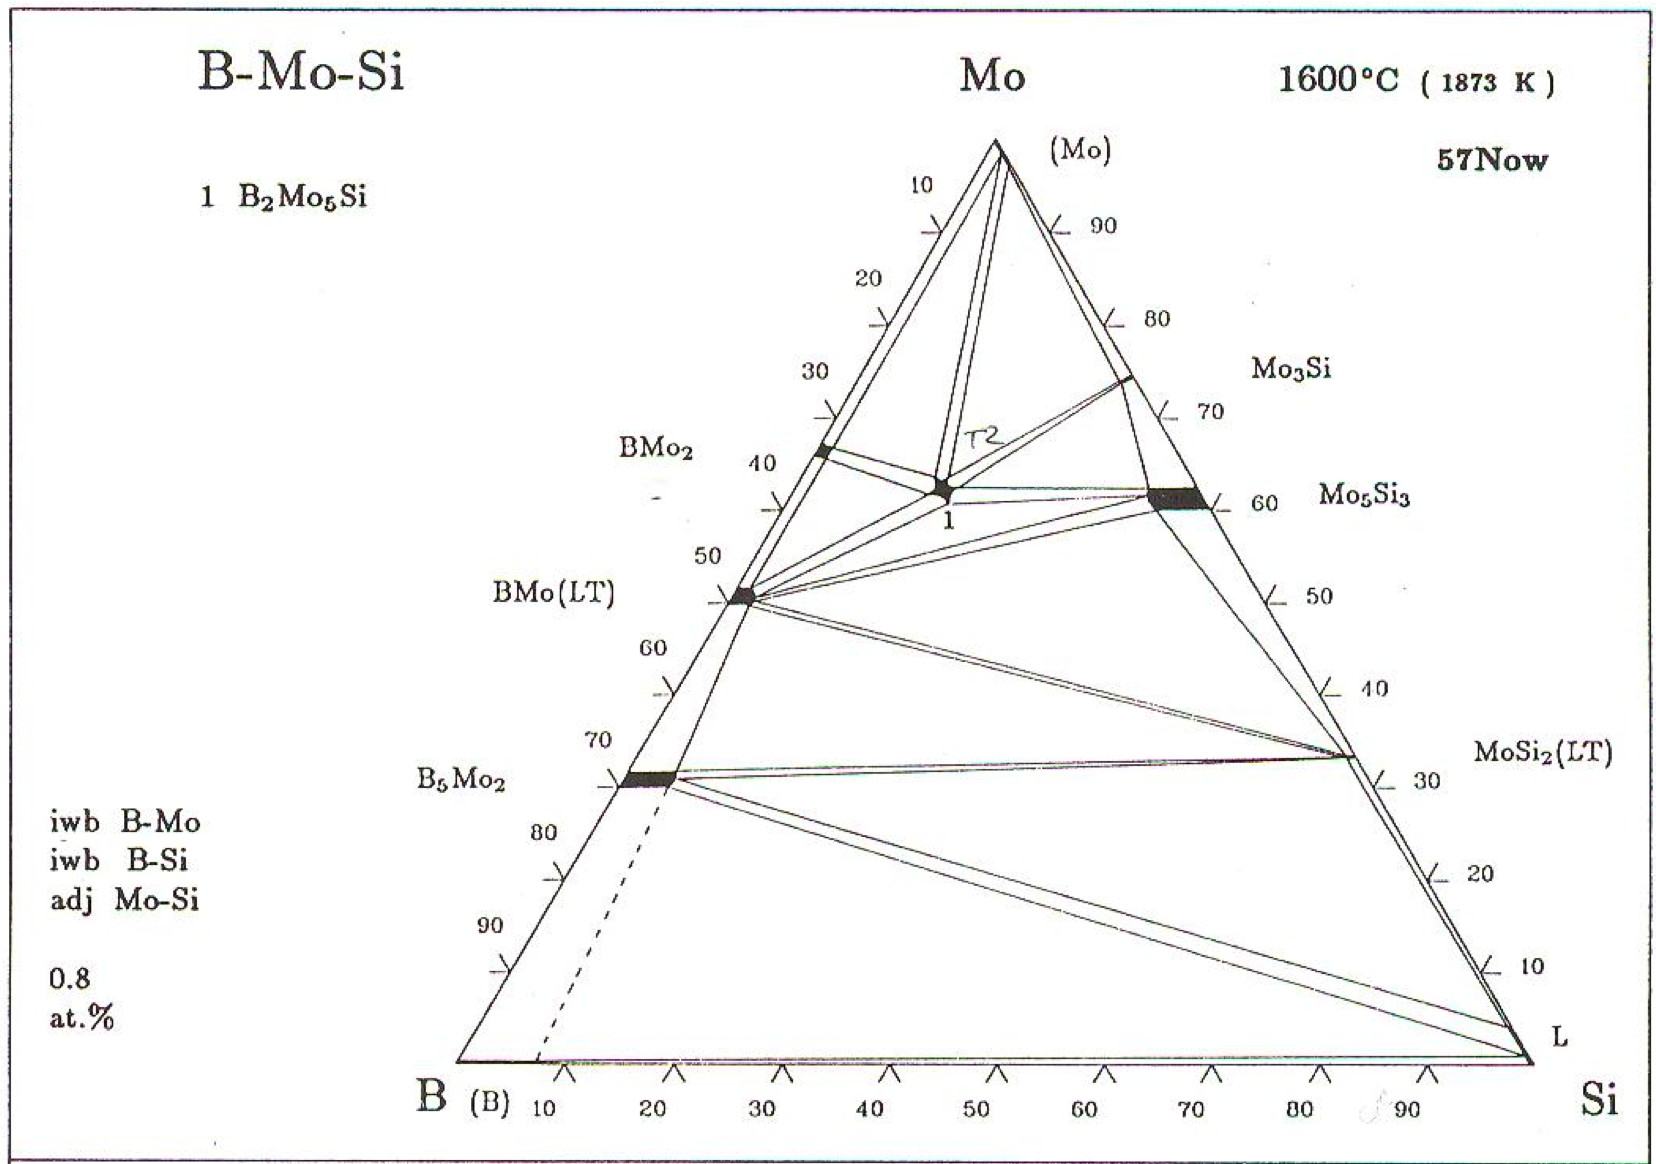
\includegraphics[width=\textwidth]{MoSiB_1600}
\caption{The ternary phase diagram of Mo--Si--B ~\cite{nowotny57}.}
\label{fig:MoSiB_1600}
\end{center}
\end{figure}
%
\begin{figure}[H]
\begin{center}
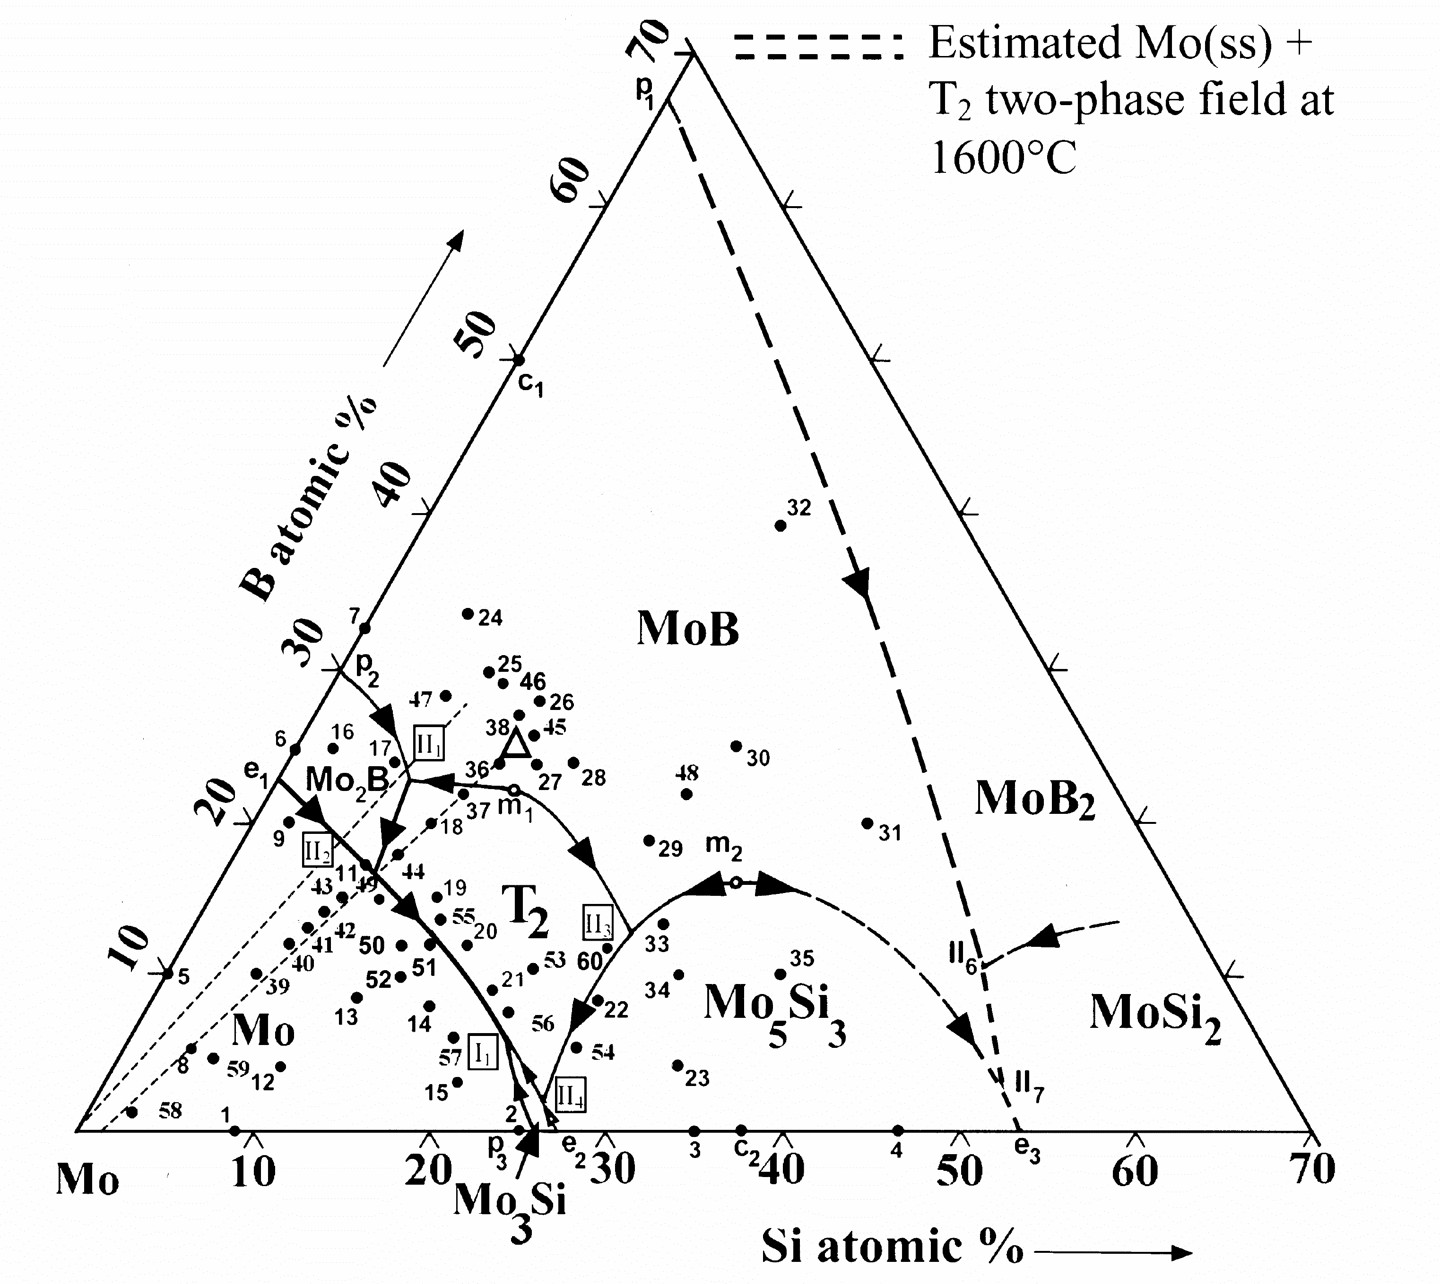
\includegraphics[width=.9\textwidth]{MoSiB_liquidus}
\vspace{-3mm}
\caption{The relevant portion of the Mo--Si--B liquidus projection T= 1873K ~\cite{perepezko01}.}\label{fig:MoSiB_liquidus}
\end{center}
\end{figure}
\vspace{-5mm} 	
%
\begin{figure}[H]
\begin{center}
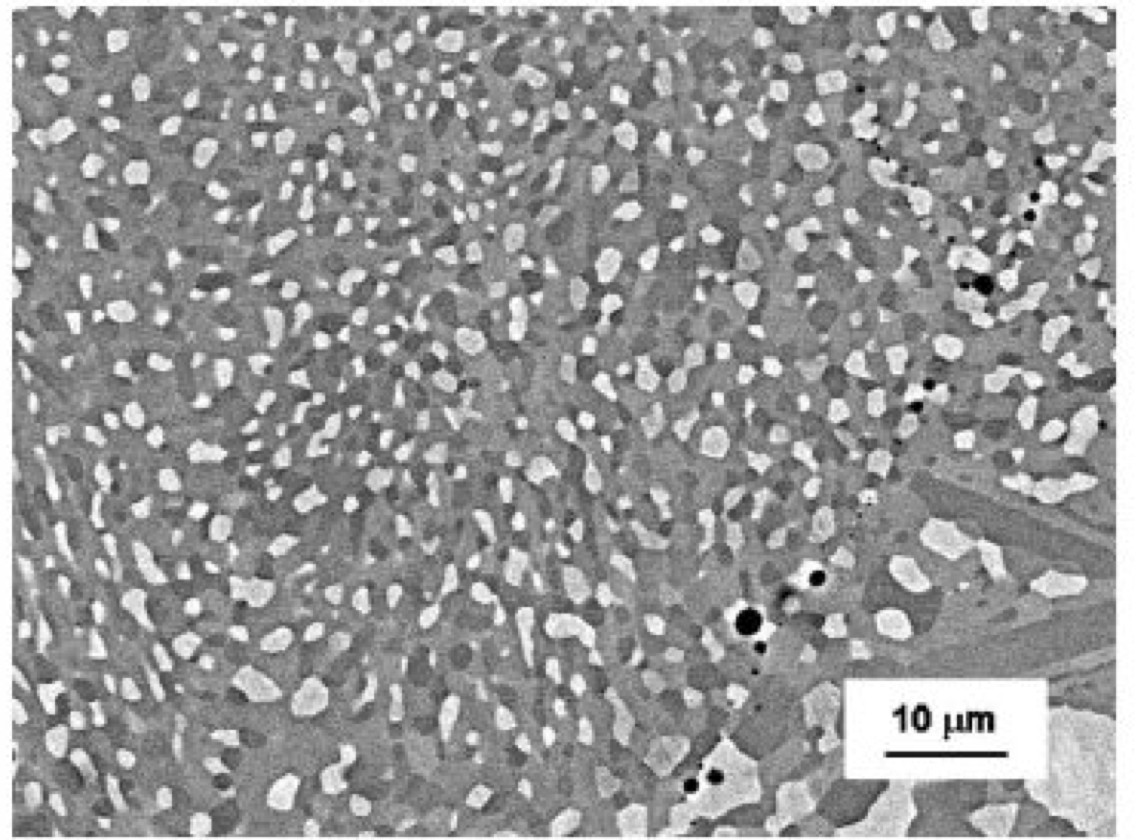
\includegraphics[width=9cm]{Mo16Si8B}
\caption{SEM micrograph of Mo--16.8Si--8.4B ~\cite{perepezko01}.}
\label{fig:Mo16Si8B}
\end{center}
\end{figure}
%
One approach that Perepezko has taken is to introduce alloying elements, such as Nb, that stabilise the T2 phase and destabilise boride reactions (Figure \ref{fig:MoSiB_withNb}) ~\cite{perepezko01, sakidja00}. Nb can subsubstitute for Mo to a large extent in solid solution and T2. This increases microstructural control and allows for direct solidification of a two-phase solid solution and T2 microstructure in the region shaded in the liquidus projection (Figure \ref{fig:Mo19Nb12Si8B}). 
%
\begin{figure}[H]
\begin{center}
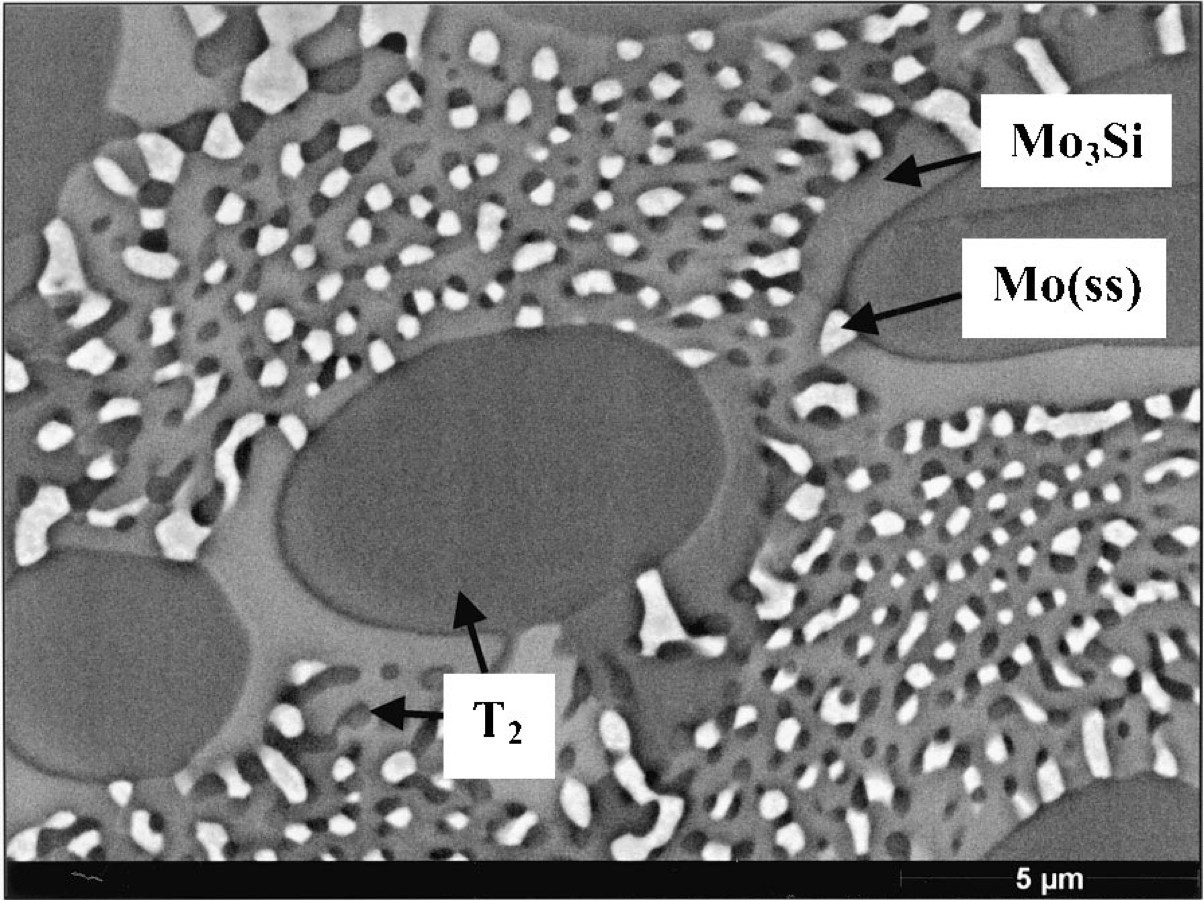
\includegraphics[width=.5\textwidth]{MoSiB_witheutectic}
\caption{T2 primary phase and Mo(ss)--T2--Mo$_3$Si invariant ternary eutectic ~\cite{perepezko01}.}
\label{fig:MoSiB_witheutectic}
\end{center}
\end{figure}
\vspace{.7cm} 
%
\begin{figure}[H]
\begin{center}
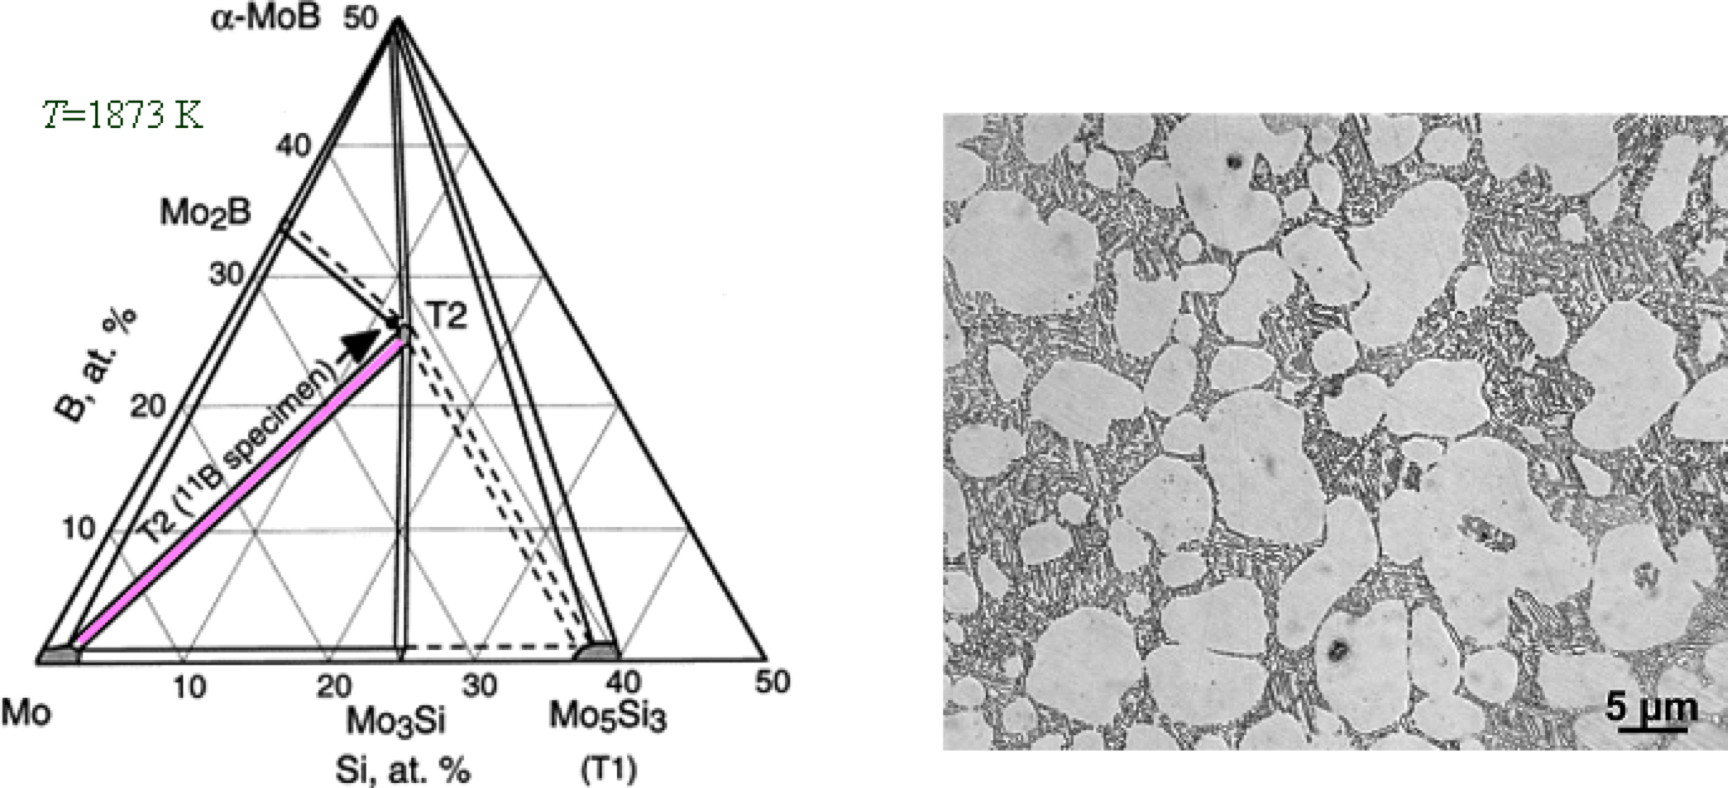
\includegraphics[width=\textwidth]{MoSiB_withNb}
\caption{Increase in solid solution volume fraction in the ternary eutectic with Nb alloying ~\cite{perepezko01}.}\label{fig:MoSiB_withNb}
\end{center}
\end{figure}
%
\begin{figure}[H]
\begin{center}
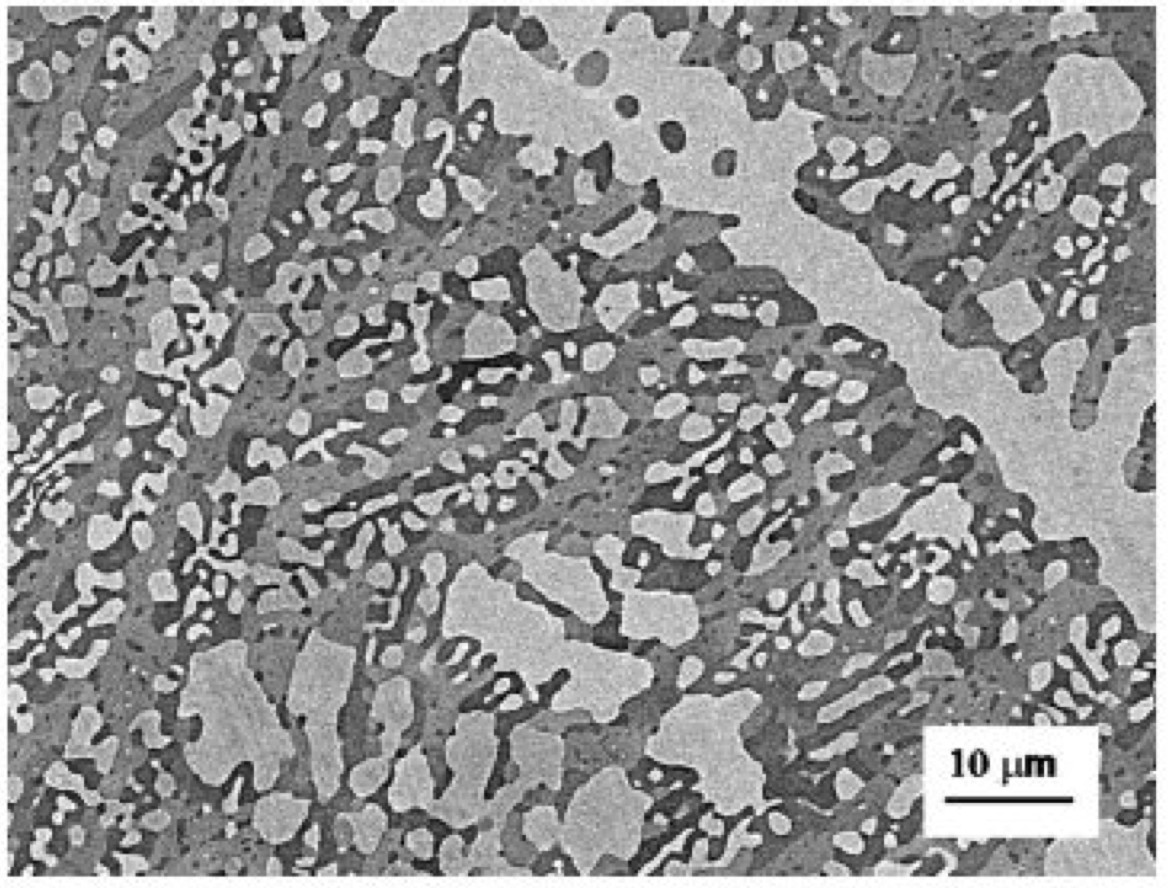
\includegraphics[width=.5\textwidth]{Mo19Nb12Si8B}
\caption{SEM micrograph of polished section of cast and annealed Mo--19.5Nb--12Si--8.5B (at.\%) ~\cite{perepezko01}.}\label{fig:Mo19Nb12Si8B}
\end{center}
\end{figure} 
%
\subsection{Niobium Silicides}
There are three niobium silicides in the Nb--Si binary: Nb$_3$Si, Nb$_5$Si$_3$ and NbSi$_2$ (Figure \ref{fig:NbSi}). Niobium has a density of 8.57 \gram\usk\centi\rpcubic\meter, and Nb$_3$Si has a density of 7.52 \gram\usk\centi\rpcubic\meter. Niobium silicides have very poor oxidation resistance, pesting at low and intermediate temperatures. They have poor room temperature fracture toughness and their pesting issues have yet to be resolved ~\cite{fleischer87,fleischer94, sauthoff88, shah92}. The eutectic between niobium solid solution and Nb$_3$Si has been looked at ~\cite{kimura05}, but there are many phase transitions between room temperature and the eutectic melting point (Figure \ref{fig:NbSi}). At 1765\celsius, Nb$_3$Si undergoes a eutectoid decomposition to Nb and Nb$_5$Si$_3$.  To further complicate matters, Nb$_5$Si$_3$ has two allotropes.

Directionally solidified Nb-Nb$_3$Si alloys have been examined by Bewlay et al. [17].  Hypoeutectic alloys have Nb dendrites with interdendritic eutectic consisting of a Nb$_3$Si matrix with fine Nb rods and ribbons aligned with the primary growth direction.   Hypereutectic alloys were found to contain primary Nb$_3$Si and Nb$_5$Si$_3$ dendrites with interdendritic eutectic.  The fracture toughnesses of these materials ranged from 5.8 \mega\pascal\usk\meter$^{\frac{1}{2}}$ at the eutectic composition to 14.2 \mega\pascal\usk\meter$^{\frac{1}{2}}$ for a hypoeutectic composition at 10 at.\% Si, which are significantly better than monolithic Nb$_5$Si$_3$.  In fact, 14.2 is close to the minimum threshold for fracture toughness of 15\mega\pascal ~\cite{shah95}.   However, the addition of the niobium matrix decreases creep strength by an order of magnitude at 1200\celsius, with minimum creep rates comparable to those of nickel-base superalloys. The eutectic (Nb,Mo)$_5$Si$_3$--Nb,Mo)s.s. system shows good high temperature mechanical properties. However, the issue of poor oxidation resistance is not addressed with molybdenum additions. Shah has reported that preliminary attempts to attain the C14 (Cr$_2$Nb--Si) phase in a Nb--Cr--Si solid solution matrix were not encouraging; this is believed to have been caused by a complex intersection of liquidus surfaces. 
%
\begin{figure}[H]
\begin{center}
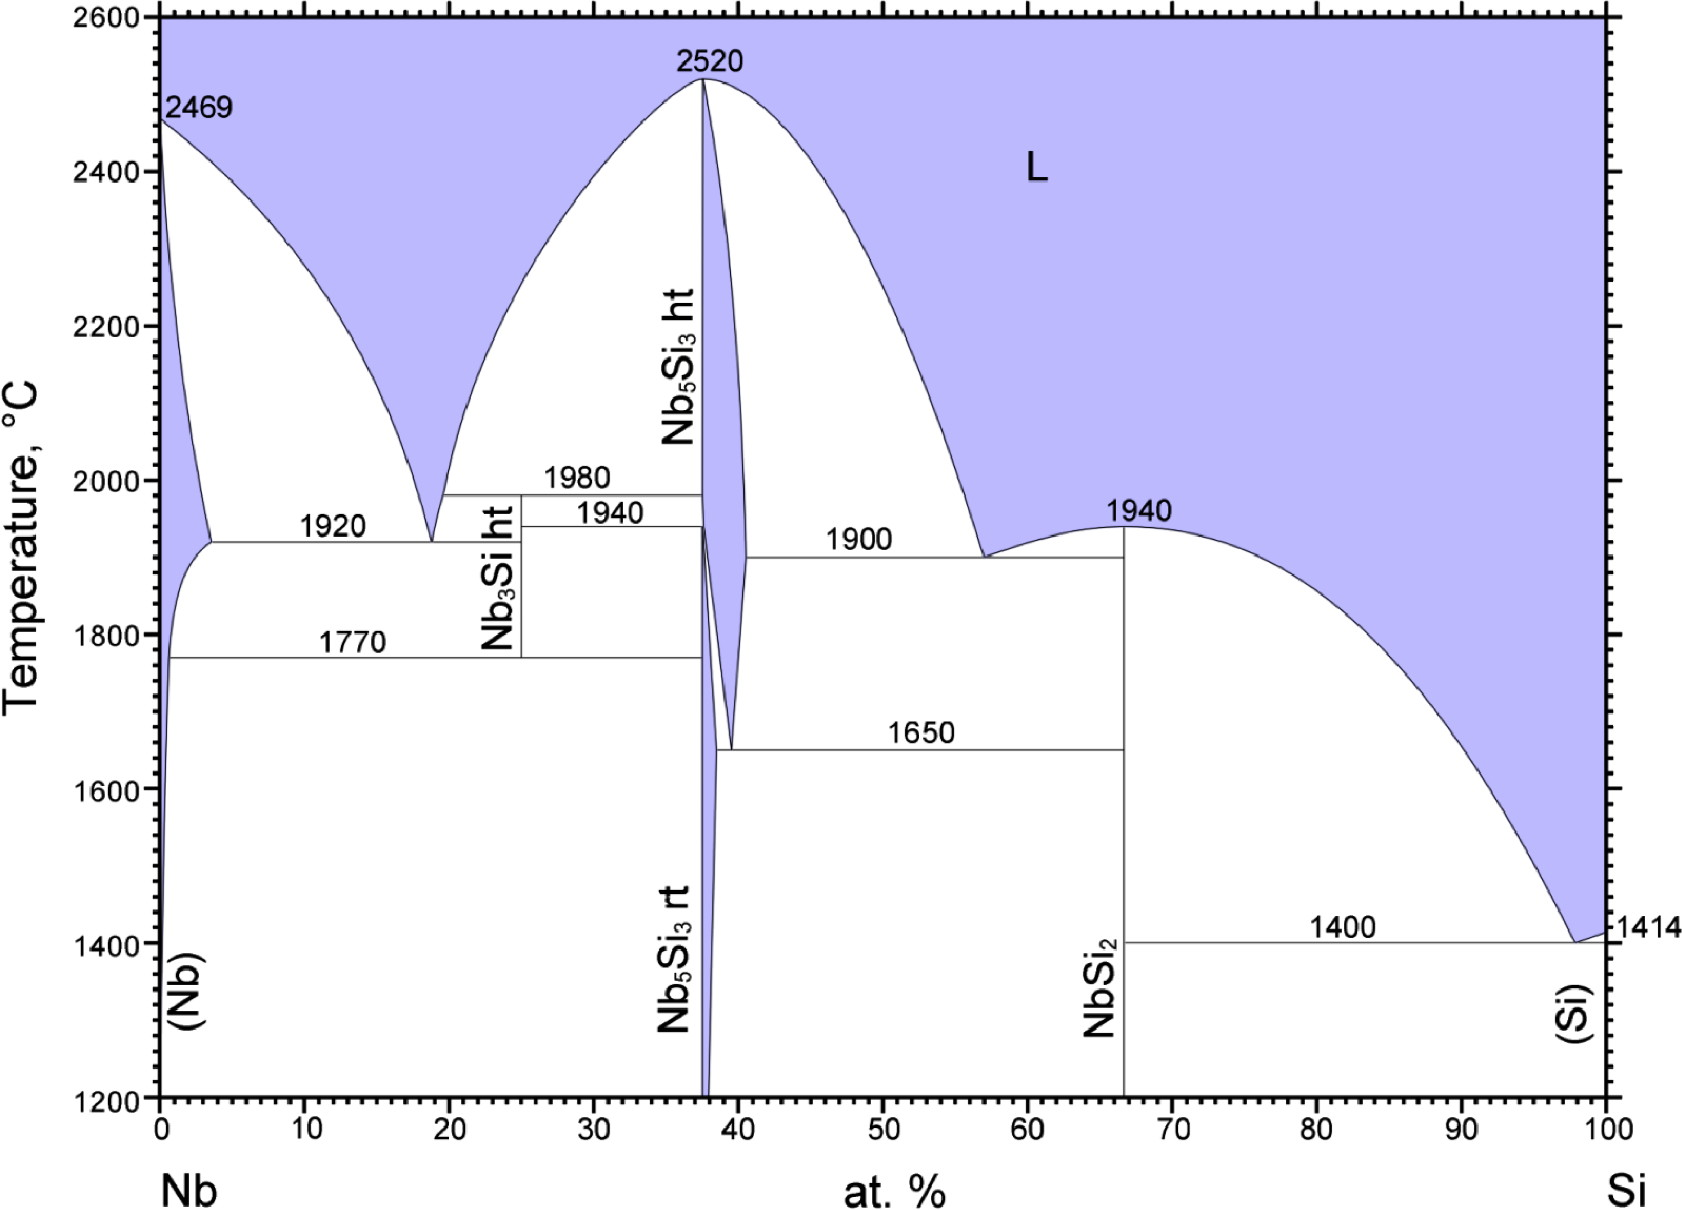
\includegraphics[width=.8\textwidth]{NbSi}
\vspace{-2mm}
\caption{The Nb--Si binary phase diagram.}\label{fig:NbSi}
\end{center}
\end{figure}  
%
\subsection{Chromium Silicides}
There are four chromium silicides in the Cr--Si binary: Cr$_3$Si, Cr$_5$Si$_3$, CrSi and CrSi$_2$ (Figure \ref{fig:CrSi}) ~\cite{gokhale90}.  We are interested in Cr$_3$Si as our strengthening phase because it is the intermetallic that can co-exist with the b.c.c. chromium solid solution phase. There has been some research conducted on Cr$_5$Si$_3$, and like other intermetallics that have not been ductile-phase toughened, it has been shown to be brittle at room temperature. The components of the chromium-silicon binary have low density. The density of the solid solution is 6.91 \gram\usk\centi\rpcubic\meter, the density of Cr$_3$Si is 6.47 \gram\usk\centi\rpcubic\meter.
The theoretical Cr$_3$Si volume fraction in the Cr-Cr$_3$Si eutectic is 42 at.\%, as predicted by the binary phase diagram (Figure \ref{fig:CrSi}). This value is much lower than the 62 at.\% reported by both H. Bei and Sutcliff et al. due to non-equilibrium solidification conditions. The sensitivity of microstructure to changes in composition and solidification rate have been detailed by H. Bei et al. (Figure \ref{fig:Cr-Cr3Si_micros}) ~\cite{bei03a}. Slight deviations in composition of less than 1 at.\% can cause the microstructure to regress from lamellar to cellular. 
%
\begin{figure}[H]
\begin{center}
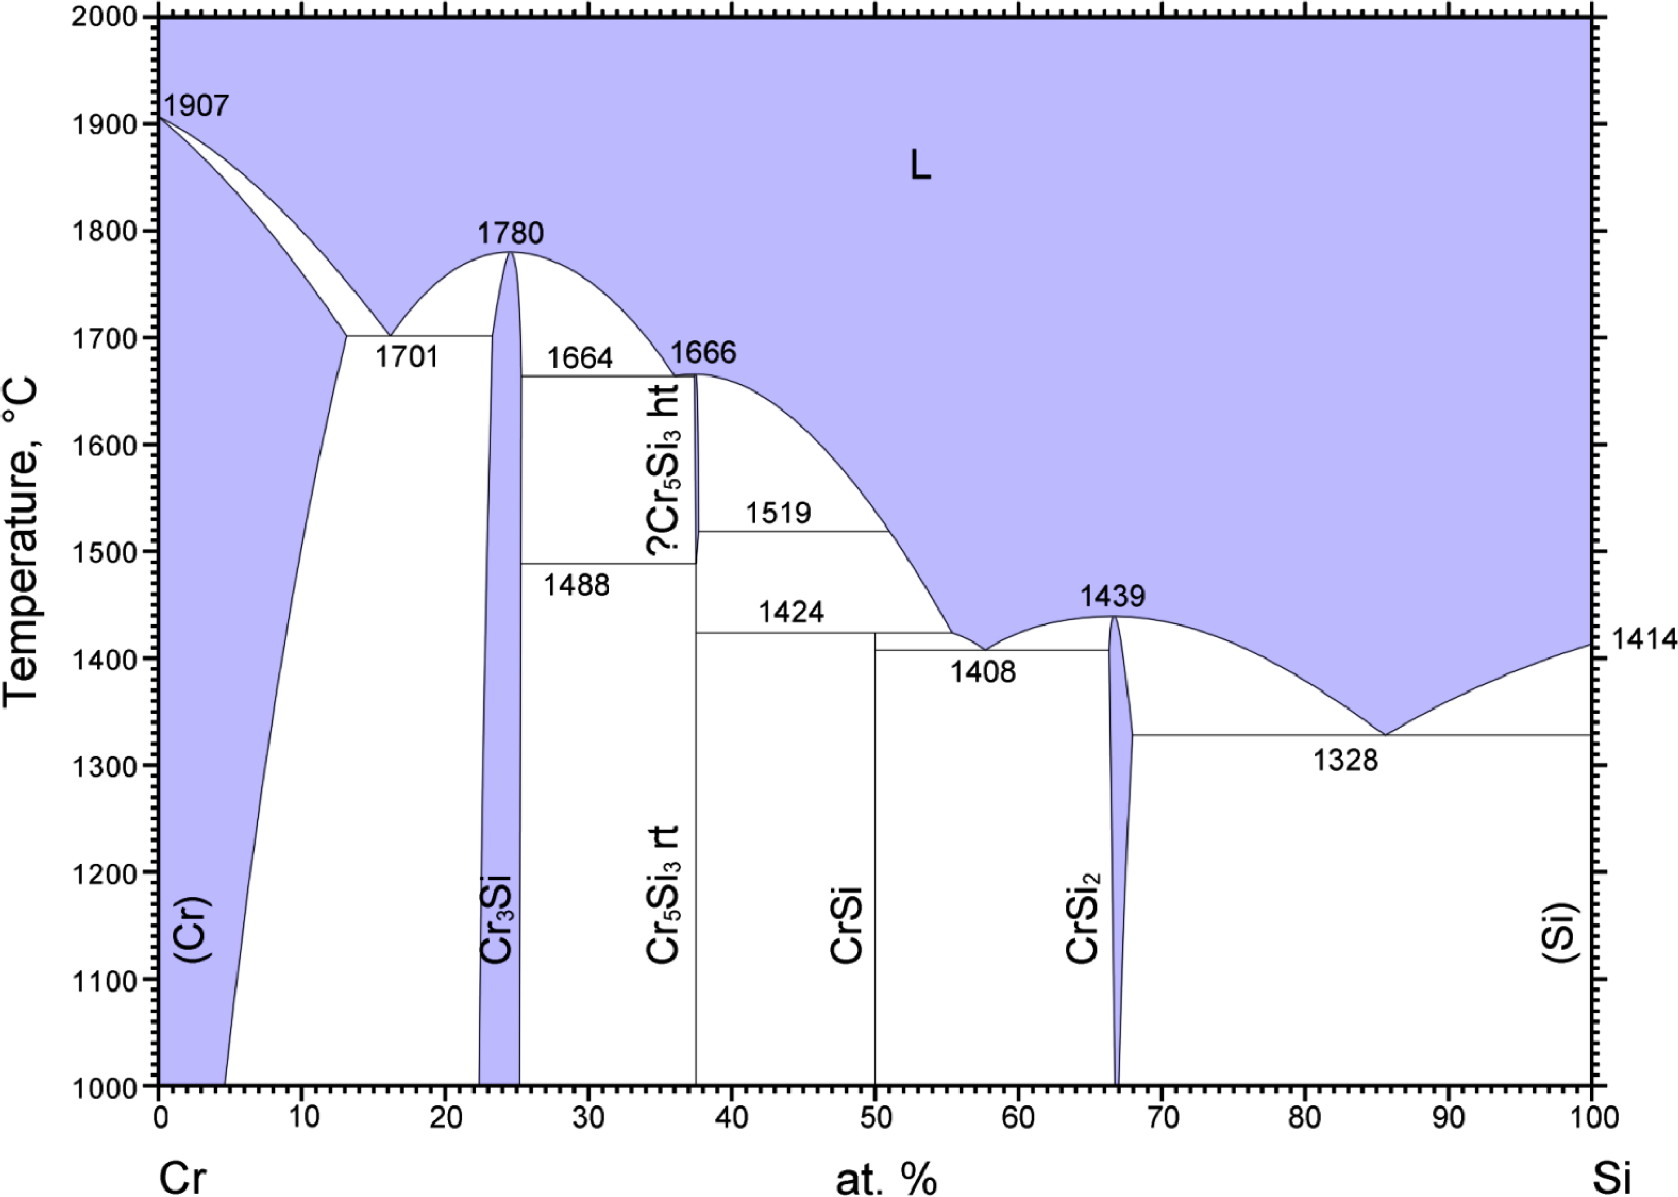
\includegraphics[width=.8\textwidth]{CrSi}
\caption{The Cr-Si binary phase diagram.}\label{fig:CrSi}
\end{center}
\end{figure}
%
\begin{figure}[H]
\begin{center}
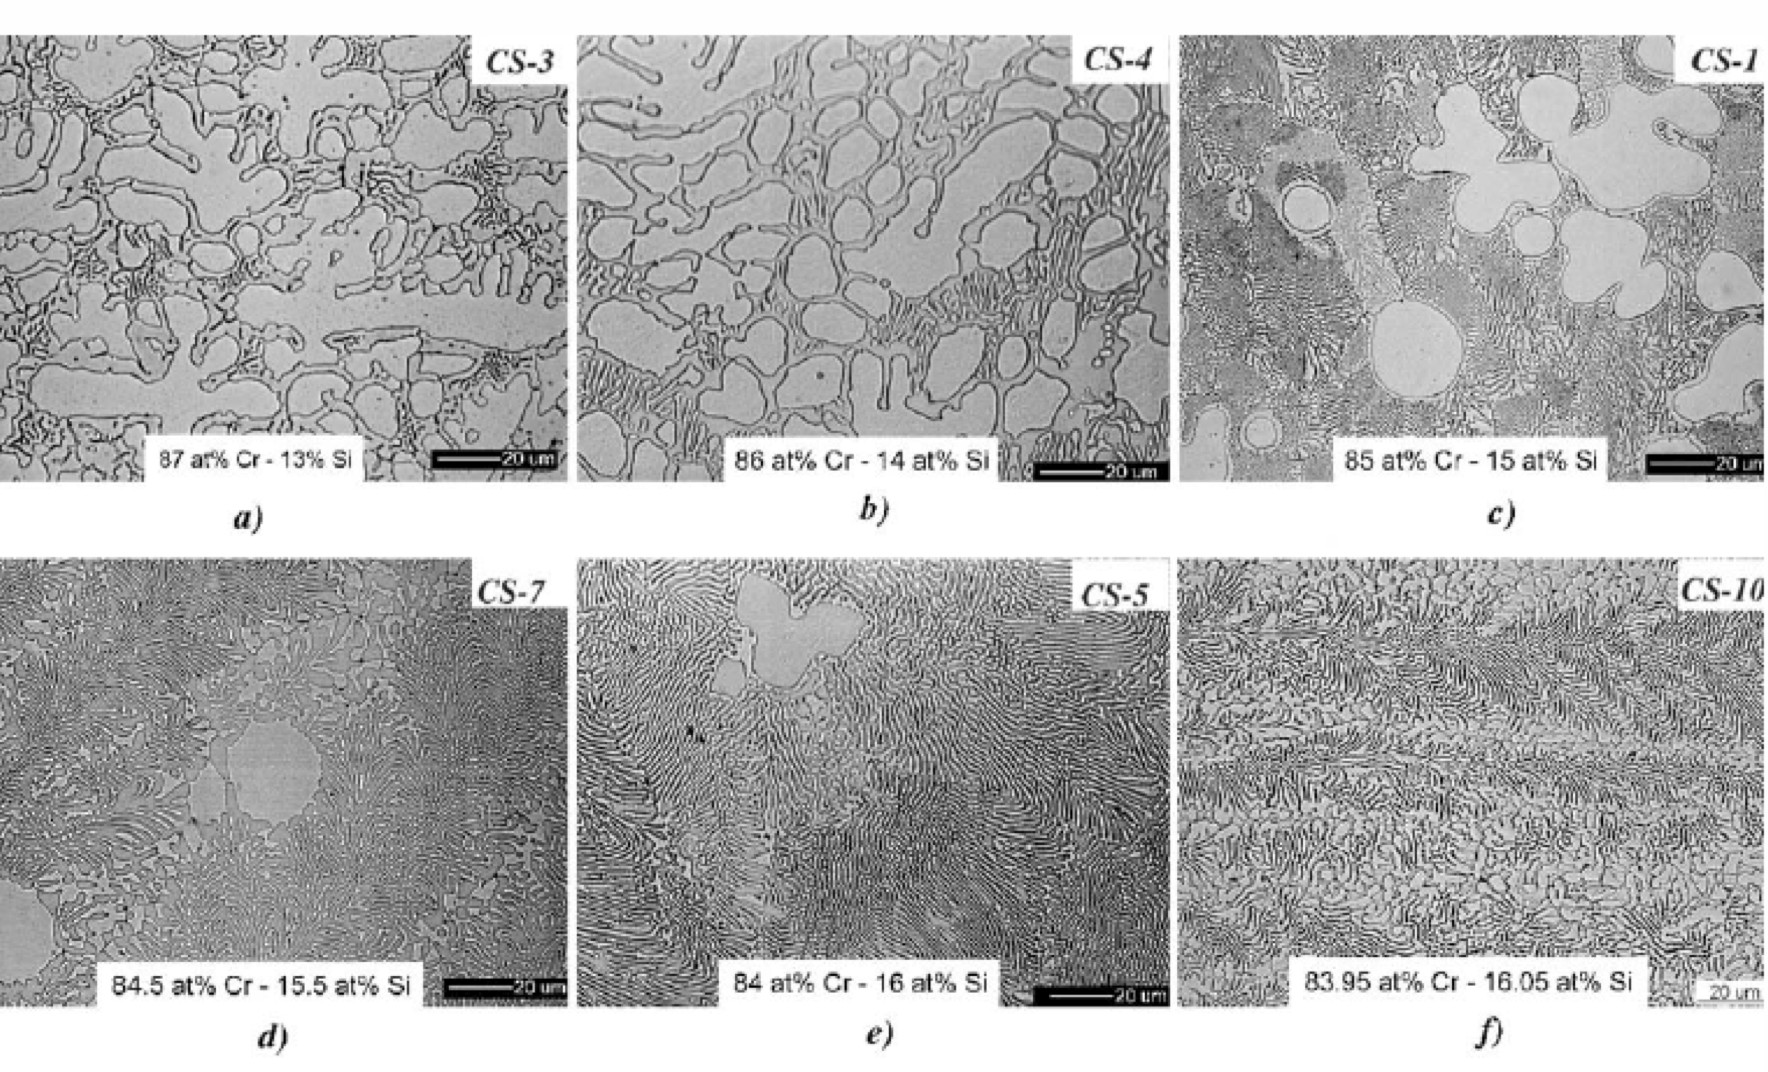
\includegraphics{Cr-Cr3Si_micros}
\caption{Changes in microstructure of Cr--Cr$_3$Si with minute deviatiations from eutectic composition ~\cite{bei03a}.}\label{fig:Cr-Cr3Si_micros}
\end{center}
\end{figure}
%
Initial evaluation of this eutectic's oxidation resistance has been conducted by several groups, and they have contradictory results.  E. Aitken reports that Cr$_3$Si has good oxidation resistance.  He observes that a dual-layer oxide scale comprising of Cr$_2$O$_3$ sitting beneath SiO$_2$ grows upon oxidation at 1200\celsius.   Raj reports Cr$_3$Si as having poor oxidation resistance above 1200\celsius ~\cite{raj95}.   When exposed for 4 hours at 1200\celsius, a Cr$_2$O$_3$ layer forms with islands of SiO$_2$ sitting on top.  After 4 hours at 1400\celsius, a layer of SiO$_2$ manages to form, but it possesses poor adhesion.  
% His opinion supports the findings of Grabke et al.
 
\subsection{Vanadium Silicides}
There are four vanadium silicides in the V--Si binary: V$_3$Si, V$_5$Si$_3$, V$_6$Si$_5$ and VSi$_2$ (Figure \ref{fig:VSi}) ~\cite{smith90}. The density of the solid solution is 6.11 \gram\usk\centi\rpcubic\meter and V$_3$Si is 5.2\gram\usk\centi\rpcubic\meter. The V solid solution melts at 1910 \celsius\  and V$_3$Si melts at 1925\celsius\ ~\cite{freund78}. Limited work has been done on V--V$_3$Si ~\cite{strum93}.
%
\begin{figure}[H]
\begin{center}
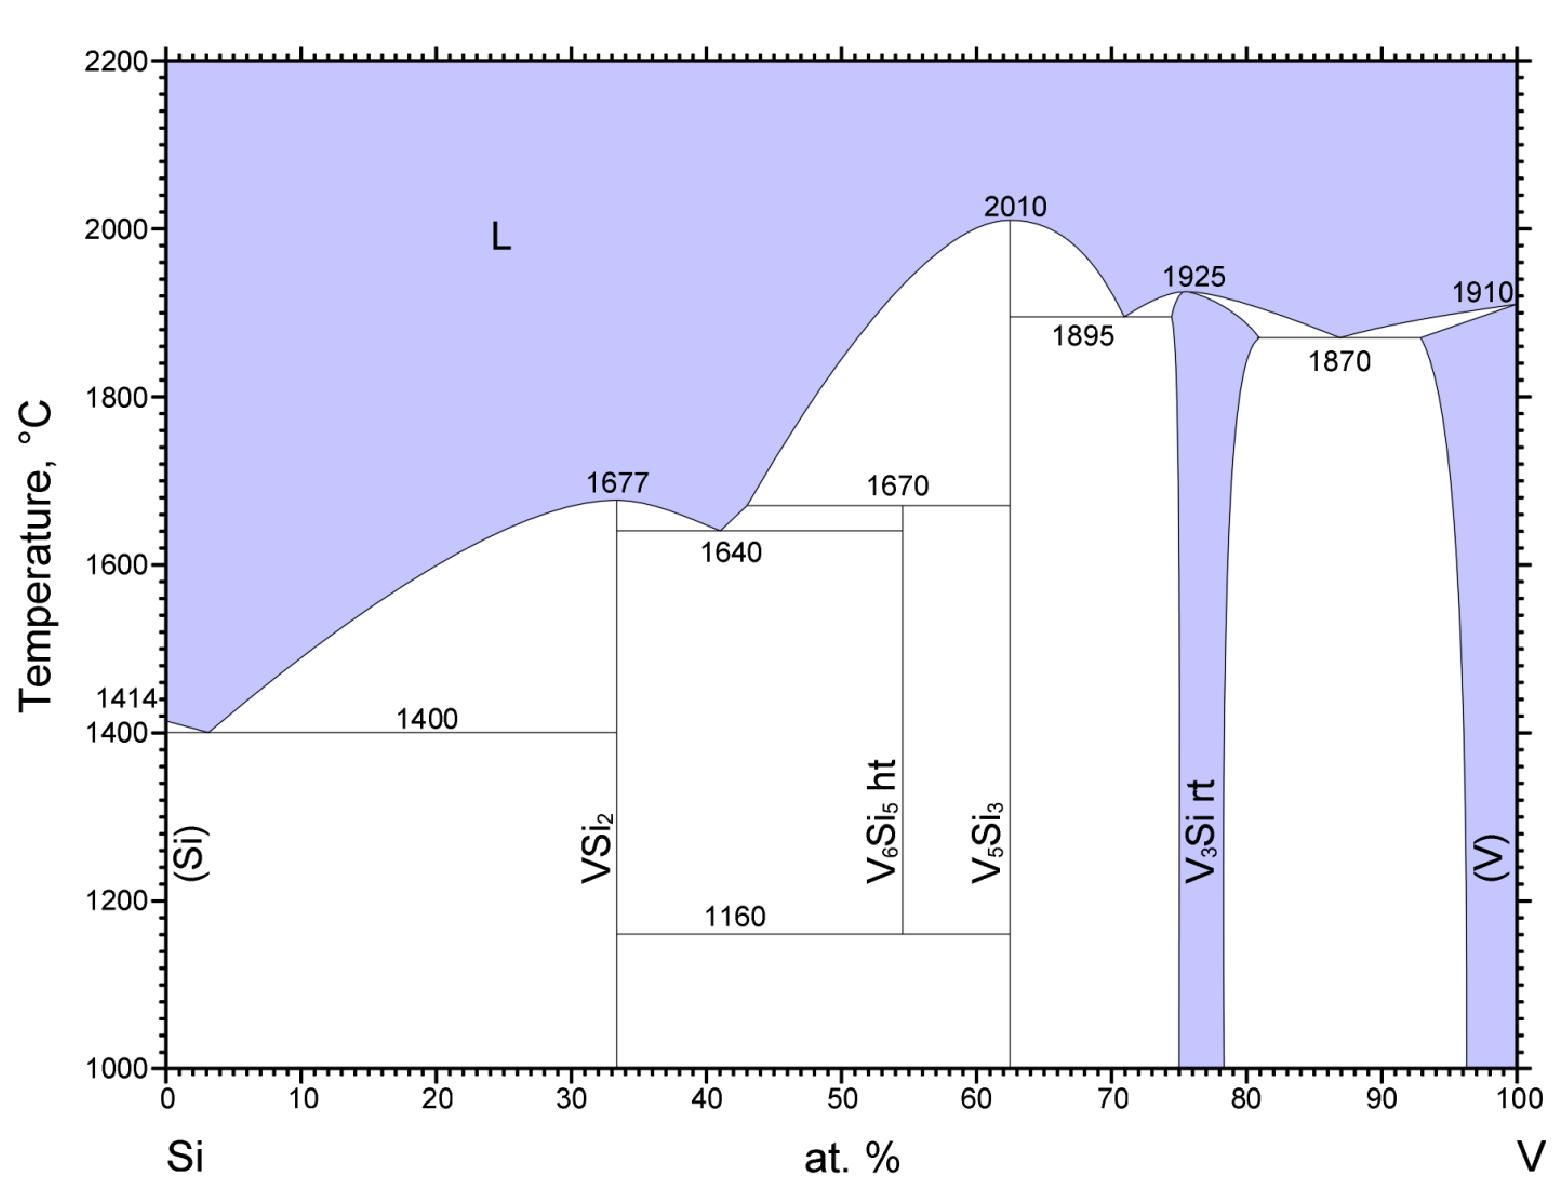
\includegraphics[width=.8\textwidth]{VSi}
\caption{The V-Si binary phase diagram ~\cite{smith90}.}
\label{fig:VSi}
\end{center}
\end{figure}
%
\subsection{Titanium Silicides}
There are five titanium silicides in the Ti--Si binary: Ti$_3$Si, Ti$_5$Si$_3$, Ti$_5$Si$_4$, TiSi and TiSi$_2$ (Figure \ref{fig:TiSi}) ~\cite{seifert96ti}. The density of the solid solution is 4.51 \gram\usk\centi\rpcubic\meter. Ti$_5$Si$_3$ has been found to have excellent density corrected high temperature properties, but, like other intermetallics, show poor fracture toughness at room temperature. The Ti solid solution melts at 1667\celsius, and cannot be considered as a matrix for a material operating over 1000\celsius.
%
\begin{figure}[H]
\begin{center}
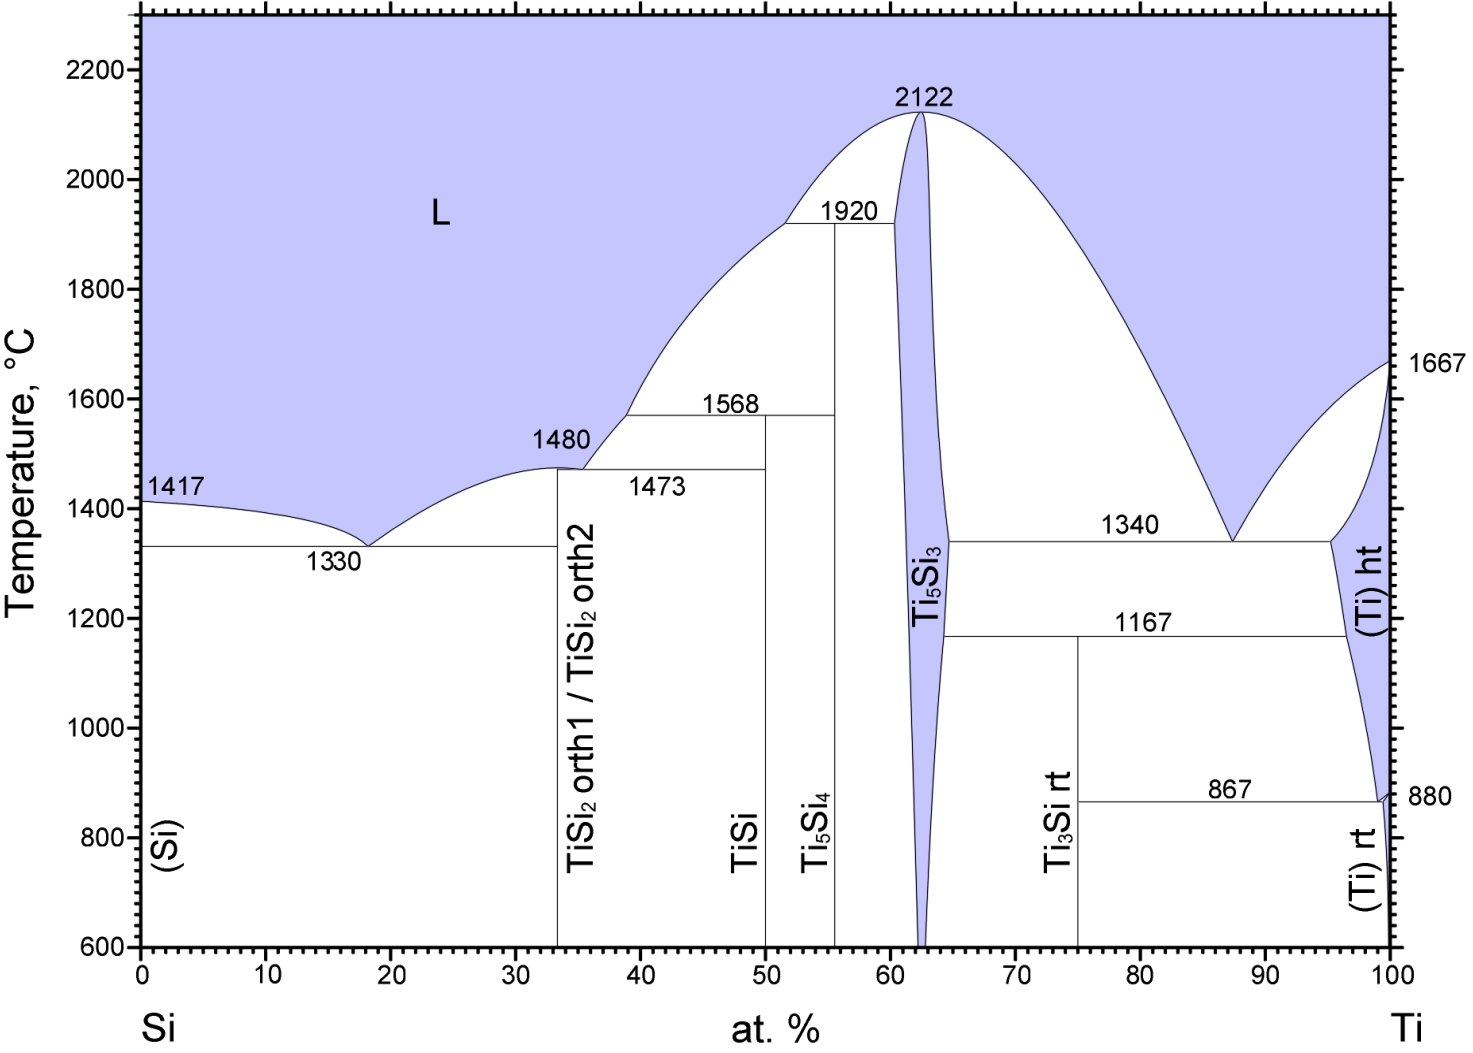
\includegraphics[width=\textwidth]{TiSi}
\caption{The Ti-Si binary phase diagram ~\cite{seifert96ti}.}\label{fig:TiSi}
\end{center}
\end{figure}
%


\section{Material Manufacture and Processing}

Intermetallics currently experience a low degree of microstructural refinement, as many have very high melting points above 2000\celsius.  The choice of casting equipment is limited for such materials; thus, a large portion of research has been performed on ingots that are arc-melted or processed by powder-metallurgy.  The presence of grain boundaries in these microstructures is disadvantageous for high temperature creep resistance. Also, the fast solidification rates experienced by arc-melted ingots can result in micro-cracks caused by thermal shock ~\cite{raj95a}.

Microstructural refinement can be achieved with specimens prepared by casting, as they will have substantially fewer grains and possess texture.  Polycrystalline directionally solidified ingots can be cast using a radio frequency furnace for materials with melting temperatures that are less than 1800\celsius.  For material that have melting points that are less than 2800\celsius, a mirror image furnace can be used to cast polycrystalline or single crystal ingots. Shah has reported that material manufacture using this technique will prove experimentally difficult ~\cite{shah95}.  Feed ingot chemistry needs to be homogenous, growth and rotation rates need to be controlled to prevent orientation misalignment.  He also thinks that directional solidification may not be sustainable for solid-solution rich or low viscosity melts.

